\documentclass{beamer}
\mode<presentation>
\usetheme{Warsaw} 
\usepackage[T1]{fontenc}
\usepackage[spanish]{babel}
\usepackage[utf8]{inputenc}
\usepackage{multicol}
\usepackage{xcolor}
\usepackage{natbib}
\usepackage{adjustbox}
\usepackage{graphicx} %to include graphics
\usepackage{pgfpages}
\usepackage[skins]{tcolorbox} %package for setting the colors for the new style of the note slides.
    %%I had to install spanish in babel package: sudo apt-get update; sudo apt-get install texlive-lang-spanish %https://howtoinstall.co/es/ubuntu/trusty/texlive-lang-spanish



%%%%%%%%%%%%%%%%%%%%%%%%%%%%%%%
%%%%%%%% INITIAL SETTINGS %%%%%
%%%%%%%%%%%%%%%%%%%%%%%%%%%%%%%

%%%%set the colors of beamer
\setbeamercolor{upcol}{fg=black,bg=blue!30}
\setbeamercolor{lowcol}{fg=black,bg=yellow!40}


%%%%Set comments in a lateral slide
%hide notes
%\setbeameroption{hide notes}

%set the notes as a second slide (in the same window)
%\setbeameroption{show notes}
    %even if you have notes in the tex file, if you annotate this line and unannote the previous one, comments will not appear in the compiled pdf.

%set only notes
%\setbeameroption{show only notes}
    %https://tex.stackexchange.com/questions/20227/beamer-compile-only-notes

%set the notes in the same slide but as a second window at the right.
%\setbeameroption{show notes on second screen=right} %for obtaining notes a the bottom
    %to add notes: \note{hola mundo}

%set the new color for the notes background
\newtcolorbox{note box}{enhanced,
    height=\paperheight,
    frame hidden,
    boxrule=0mm,
    colback=bg, % note background color defined by beamer 
    arc=0mm,
    grow to left by=1cm,
    grow to right by=1cm,
} %https://tex.stackexchange.com/questions/559109/beamer-remove-the-header-of-notes-section-but-keep-the-background-color

%set the new style for the notes using the new note box created previously. We do not want the current slide in the note slide.
\setbeamertemplate{note page}{% 
               \begin{note box}
                 \insertnote %put here the notes of the correspoding slide. 
               \end{note box}
} %https://tex.stackexchange.com/questions/559109/beamer-remove-the-header-of-notes-section-but-keep-the-background-color

%in case you want the slide previw in the note slides
%\setbeamertemplate{note page}{
        %\insertslideintonotes{0.5}
        %\rule{\textwidth}{0.1pt}
        %\color{blue}
        %\scriptsize \small
        %\insertnote
%} %https://tex.stackexchange.com/questions/546729/how-to-share-a-beamer-pdf-by-teleconference-zoom-etc-using-the-show-notes-on
%\setbeamercolor{note page}{bg=white!90!black, fg=black}
%\setbeamercolor{note title}{bg=white!80!black, fg=black}
%\setbeamercolor{note date}{parent=note title}

%set the font size in the notepage as large
\setbeamerfont{note page}{size=\large}

%Define the font size also for subitems in notes with
\addtobeamertemplate{note page}{\setbeamerfont{itemize/enumerate subbody}{size=\large}}{}
    %https://tex.stackexchange.com/questions/61647/beamer-changing-font-size-in-notes-when-using-setbeameroptionshow-notes-on-s


%%%%Title page
%%title 
\title[]{\textbf{Improving genetic prediction for genetic-testing consumers}}

%set space
\vspace{-0.3cm}

%%author
\author[Diego F. Salazar Tortosa (University of Arizona)]{\inst{}\\[1ex] {\LARGE \textbf{Diego F. Salazar-Tortosa}\inst{}}} 
    %Separate lines for indicating the supervisor: Seen in "https://tex.stackexchange.com/questions/26833/supervisor-field-on-the-page-of-the-title-with-beamer". 
    %alternative
        %\author[]{Diego F. Salazar-Tortosa} %los corchetes es para el texto que queda en la parte izquierda inferior negra. 

%%institute
\institute{

    %set space
    \vspace{-0.3cm}
    
    %lab
    %Enard lab
    
    %set space
    \vspace{0.2cm}
    
    %department
    %Department of Ecology and Evolutionary Biology
    
    %space
    \vspace{0.00cm}

    %University logo
    \begin{center}
    \includegraphics[width=0.27\paperwidth,height=0.32\paperheight]{figures/ua_stack_rgb_4_0.png} %downloaded from "https://brand.arizona.edu/download/full-color"
    \end{center}
} 


%%%%date
%%set the date
\date{\vspace{-1cm}February 2, 2022} %we add vspace to move the date to the bottom and avoid showing it.


%%%%Set a new environment for blocks in order to controls their width
\newenvironment<>{varblock}[2][.9\textwidth]{%
  \setlength{\textwidth}{#1}
  \begin{actionenv}#3
    \def\insertblocktitle{#2}
    \par
    \usebeamertemplate{block begin}}
    {\par
    \usebeamertemplate{block end}
  \end{actionenv}}


%%%%%Set a new title for including the title at the beginning of each chapter. Script obtained from: "https://tex.stackexchange.com/questions/311247/add-title-at-the-beginning-of-the-slide"
\makeatletter
\setbeamertemplate{title}
{
    \ifbeamercolorempty[bg]{frametitle}{}{\nointerlineskip}%
    \@tempdima=\textwidth%
    \advance\@tempdima by\beamer@leftmargin%
    \advance\@tempdima by\beamer@rightmargin%
    \vskip1ex
    \begin{beamercolorbox}[sep=8pt,center,colsep=-4bp,rounded=true]{frametitle}
        \usebeamerfont{frametitle}%
        \vbox{}\vskip-1ex%
        \if@tempswa\else\csname beamer@ftecenter\endcsname\fi%
        \strut\insertframetitle\strut\par%
        {%
            \ifx\insertframesubtitle\@empty%
            \else%
            {\usebeamerfont{framesubtitle}\usebeamercolor[fg]{framesubtitle}\insertframesubtitle\strut\par}%
            \fi
        }%
        \vskip-1ex%
        \if@tempswa\else\vskip-.3cm\fi% set inside beamercolorbox... evil here...
    \end{beamercolorbox}%
}
\makeatother


%%%%customize the footline of all slides. I only want two elements (names (instituion) and date-number slide), but you have also commented code for adding another section in the center with the short title of the talk. You only have to reduce the width (wd) to 0.333 for all sections. ht and dp are the height and the depth of the box, respectively. You would have also to change position with center/left/right. Script taken from: https://tex.stackexchange.com/questions/183339/add-author-name-short-title-date-and-pages-to-footline
\setbeamertemplate{footline}
{
    \leavevmode%
    \hbox{%
        \begin{beamercolorbox}[wd=0.5\paperwidth,ht=2.25ex,dp=1ex,center]{author in head/foot}%
            \usebeamerfont{author in head/foot}\insertshortauthor
        \end{beamercolorbox}%
        %\begin{beamercolorbox}[wd=.333333\paperwidth,ht=2.25ex,dp=1ex,center]{title in head/foot}%
            %\usebeamerfont{title in head/foot}\insertshorttitle
        %\end{beamercolorbox}%
        \begin{beamercolorbox}[wd=0.5\paperwidth,ht=2.25ex,dp=1ex,right]{date in head/foot}%            
            \usebeamerfont{date in head/foot}\insertshortdate{}\hspace*{2em}
            \insertframenumber{} / \inserttotalframenumber\hspace*{2ex} 
        \end{beamercolorbox}}%
        \vskip0pt%
    }
\makeatother


%%%%create new commands to avoid that backup slides count for the counter of slides at the bottomright of each slide.
\newcommand{\backupbegin}{%begin backup frames
   \newcounter{finalframe}
   \setcounter{finalframe}{\value{framenumber}}
}
\newcommand{\backupend}{%end backup frames
   \setcounter{framenumber}{\value{finalframe}}
}%before this command you have to add the command \appendix. Script taken from https://tex.stackexchange.com/questions/70448/dont-count-backup-slides 


%%%%For removing navigation symbols in beamer
\beamertemplatenavigationsymbolsempty%See "https://tex.stackexchange.com/questions/686/how-to-get-rid-of-navigation-symbols-in-beamer"


%%%%Notes:

%Inside the notes
    %the first itemize point is the script, the rest are additional annotations. 
    %In that script, pronunciation of some words is shown between brackets and with "". Also advice for selecting some parts of the slide with the laser pointer are included. 
    %The second point will be information about the figure in the slide or additional comments.



%%%%%%%%%%%%%%%%%%%%%%%%%%%%%%%
%%%%%%%% BEGIN SLIDES %%%%%%%%%
%%%%%%%%%%%%%%%%%%%%%%%%%%%%%%%
\begin{document}



%%%%%%%%%%%%%%%%%%%%%%%%%%%%%%%%%%%%%%%%%%%%%%%
%%%%%%%% TITLE PAGE FOR PREVIOUS WORK  %%%%%%%%
%%%%%%%%%%%%%%%%%%%%%%%%%%%%%%%%%%%%%%%%%%%%%%%
\begin{frame} 
    
    %add the title page
    \titlepage
\end{frame}


%%%%%%%%%%%%%%%%%%%%%%%%%%
%%%%%%%% NEW FRAME %%%%%%%
%%%%%%%%%%%%%%%%%%%%%%%%%%

%begin frame with title
\begin{frame}{Improving genetic prediction for genetic-testing consumers}

    %begin block without title
    \begin{block}{Relevance of genetics}

        %begin list of items
        \begin{itemize}
            \item{Well known influence for some traits aside the environment}
            \item{Gaps in the knowledge of specific genetic determinants}
            \item{Limited genetic prediction of traits}
        \end{itemize}
    \end{block} %in case you want showing a block each time: https://tex.stackexchange.com/questions/67264/overlay-of-blocks-in-beamer

    %begin centered figure
    \begin{figure}
        \begin{center}

            %add spaces to set the figure in the correct place
            \vspace*{-0.5cm}

            %add figure
            \hspace*{1.75cm}\onslide<1>\includegraphics[page=1, trim={0 0 0 0}, clip=true, width=0.7\paperwidth,height=0.5\paperheight]{figures/gene_trait.png}
            \vspace*{0cm}
            
            %add footnote
            \vspace*{-0.5cm}\hspace*{0.2cm}\scriptsize Schematic representation of gene-trait relationship
        \end{center}            
    \end{figure}
\end{frame}



%%%%%%%%%%%%%%%%%%%%%%%%%%
%%%%%%%% NEW FRAME %%%%%%%
%%%%%%%%%%%%%%%%%%%%%%%%%%

%begin frame with title
\begin{frame}{Improving genetic prediction for genetic-testing consumers}

    %begin block without title
    \begin{block}{openSNP: genetic prediction of height}

        %begin list of items
        \begin{itemize}
            \item{Open-access database with genetic and height data}
            \item{5.7 GB of genetic and height data scrapped with API}
            \item{$\approx$10 thousand genetic variants associated with height}
        \end{itemize}
    \end{block} %in case you want showing a block each time: https://tex.stackexchange.com/questions/67264/overlay-of-blocks-in-beamer 

    %begin centered figure
    \begin{figure}
        \begin{center}

            %add spaces to set the figure in the correct place
            \vspace*{-0.5cm}

            %add figure
            \hspace*{1.75cm}\onslide<1>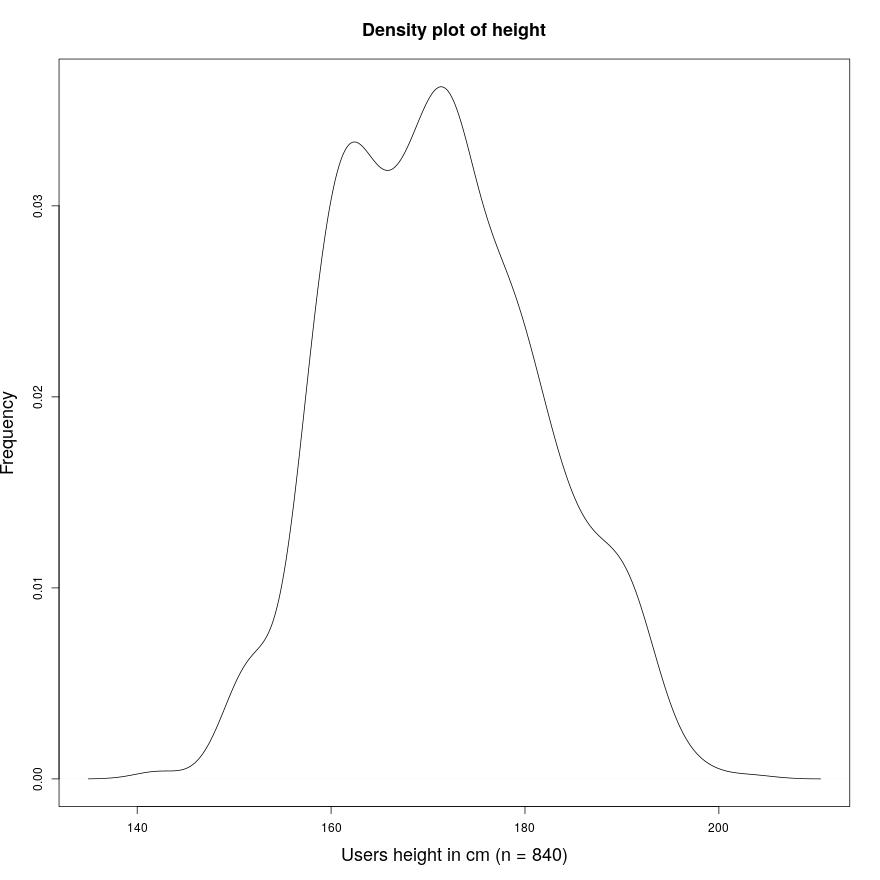
\includegraphics[page=1, trim={0 0 0 0}, clip=true, width=0.5\paperwidth,height=0.5\paperheight]{figures/height_density_plot.jpeg}
            \vspace*{0cm}
            
            %add footnote
            \vspace*{-0.5cm}\hspace*{0.2cm}\scriptsize User's height relationship
        \end{center}            
    \end{figure}
\end{frame}



%%%%%%%%%%%%%%%%%%%%%%%%%%
%%%%%%%% NEW FRAME %%%%%%%
%%%%%%%%%%%%%%%%%%%%%%%%%%

%begin frame with title
\begin{frame}{Improving genetic prediction for genetic-testing consumers}

    %begin block without title
    \begin{block}{Genetic algorithms to predict height}

        %begin list of items
        \begin{itemize}
            \item{Genetic algorithms selecting most explanatory variants}
                \begin{itemize}
                    \item{Filtering by p-value thresholds}
                    \item{Considering functional impact on proteins}
                \end{itemize}
            \item{Fine tuning of algorithm parameters -> battery of algorithms}
            \item{Quantify influence of parameters on height prediction}
        \end{itemize}
    \end{block} %in case you want showing a block each time: https://tex.stackexchange.com/questions/67264/overlay-of-blocks-in-beamer 

    %begin centered figure
    \begin{figure}
        \begin{center}

            %add spaces to set the figure in the correct place
            \vspace*{-0.5cm}

            %add figure
            \hspace*{1.75cm}\onslide<1>\includegraphics[page=1, trim={0 0 0 0}, clip=true, width=0.6\paperwidth,height=0.4\paperheight]{figures/gene_trait.png}
            \vspace*{0cm}
            
            %add footnote
            \vspace*{-0.5cm}\hspace*{0.2cm}\scriptsize Schematic representation of gene-trait relationship
        \end{center}            
    \end{figure}
\end{frame}



%%%%%%%%%%%%%%%%%%%%%%%%%%
%%%%%%%% NEW FRAME %%%%%%%
%%%%%%%%%%%%%%%%%%%%%%%%%%

%begin frame with title
\begin{frame}{Improving genetic prediction for genetic-testing consumers}

    %begin block without title
    \begin{block}{Proof of concept}

        %begin list of items
        \begin{itemize}
            \item{Improvement of algorithms for genetic prediction}
            \item{Future test on larger datasets with clinical data}
            \item{More robust predictions of disease risk for genetic-testing consumers}
        \end{itemize}
    \end{block} %in case you want showing a block each time: https://tex.stackexchange.com/questions/67264/overlay-of-blocks-in-beamer
\end{frame}
\end{document}



%%%%%%%%%%%%%%%%%%%%%%%%%%%%%%%%%%%%%%%%%%
%%%%%%%%%%%%%%% COMMAND TO RUN %%%%%%%%%%%
%%%%%%%%%%%%%%%%%%%%%%%%%%%%%%%%%%%%%%%%%%

%pdflatex seminar_v1.tex 